% !TEX root = main.tex
%%%%%%%%%%%%%%%%%%%%%%%%%%%%%%%%%%%%%%%%%%%%%%%%%%%%%%
\section{序論}
%%%%%%%%%%%%%%%%%%%%%%%%%%%%%%%%%%%%%%%%%%%%%%%%%%%%%%
\subsection{始めに}
 人工衛星とは,地球の周りをまわっている人工物体のことをいい,搭載しているセンサなどで地球の気象や地表・海面の温度,植物の有無などを調べる地球観測衛星,
位置情報を正確に測る測位衛星,インターネットなどを構成する通信衛星などがある.
内閣府の調査によれば,2023年に打ち上げられた人工衛星等の機数は,過去最大の2,901機であり,10年前と比べて約14倍に増加したという\cite{intro1}.
数十~数千の人工衛星を一体的に運用しネットワークを形成する,メガコンステレーションの構築への取り組みや,
先進国・新興宇宙開発国による,安全保障分野におけるミサイル防衛や宇宙領域把握を目的とする衛星の打ち上げも見込まれることから,宇宙輸送のニーズは一層拡大することが見込まれている.


\subsection{超小型人工衛星とは}
 人工衛星は,大きいものでは例えば大きさが約108.5 m×72.8 m 質量約420 t のISS(International Space Station)がある\cite{intro2}.
それに対し小さいものでは,一辺10 cm の立方体サイズの超小型人工衛星が存在している.
超小型人工衛星の定義は明確には決まっておらず,全質量が100 kg 以下とするものや,50 kg 以下とするものもある.
本研究では,超小型人工衛星の中でも,一辺10 cm の立方体を1Uとして規格化された小型衛星(CubeSat)に絞って述べる.
大型人工衛星,中型人工衛星と呼ばれる人工衛星は,多くが国家プロジェクトとして開発され,打ち上げられている.
その特徴として,高機能で信頼性が高く,複雑な用途,複数のミッションに活用できるという利点がある.
しかし,設計・製造に莫大な費用と時間が必要となる.
反対に,超小型人工衛星は,機能が制限され,単一のミッションしか実行できないという欠点がある.
その代わり,短期間での開発・低コストでの打ち上げが可能であるため,
学生が在学中に開発・打ち上げをすることが可能となっている.
また,世界各国が宇宙開発研究でしのぎを削るなか,新しい技術を素早く試せることも,
注目されている一つの理由である.
超小型人工衛星の,中でもCubuSatの写真を図\ref{fig:a}\cite{micro}に,中型人工衛星の写真を図\ref{fig:b}\cite{medium}に,大型人工衛星の写真を図\ref{fig:c}\cite{large}に示す.

\begin{figure}[H]
    \centering
    \begin{minipage}[b]{0.47\columnwidth}
        \centering
        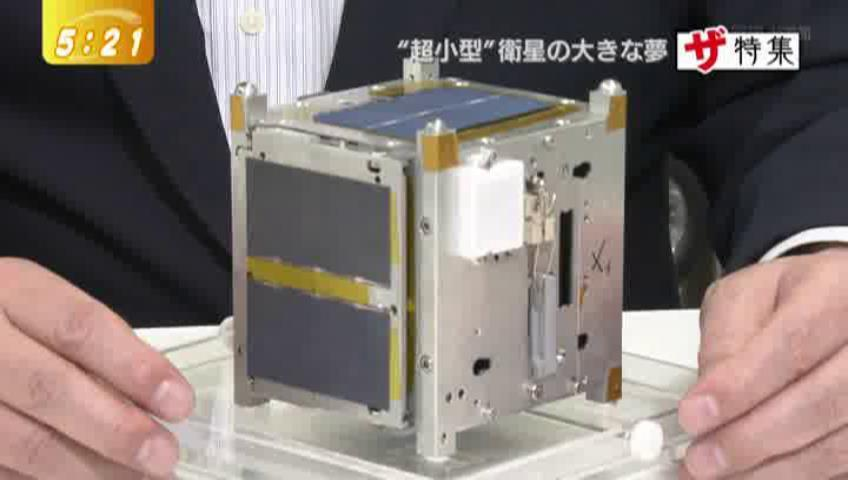
\includegraphics[width=0.9\columnwidth]{./figure/超小型.jpg}
        \caption{超小型人工衛星}
        \label{fig:a}
        \vfill
        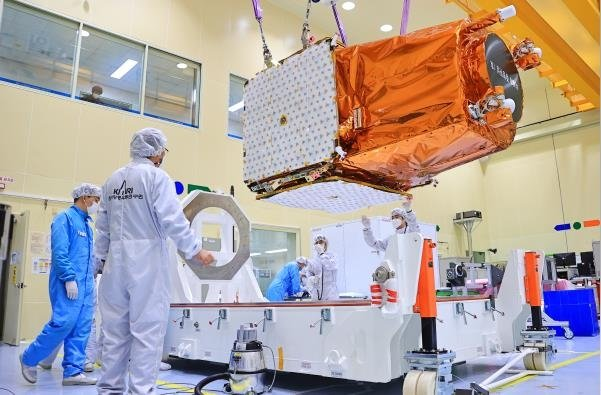
\includegraphics[width=0.9\columnwidth]{./figure/中型.jpg}
        \caption{中型人工衛星}
        \label{fig:b}
    \end{minipage}
    \begin{minipage}[b]{0.51\columnwidth}
        \centering
        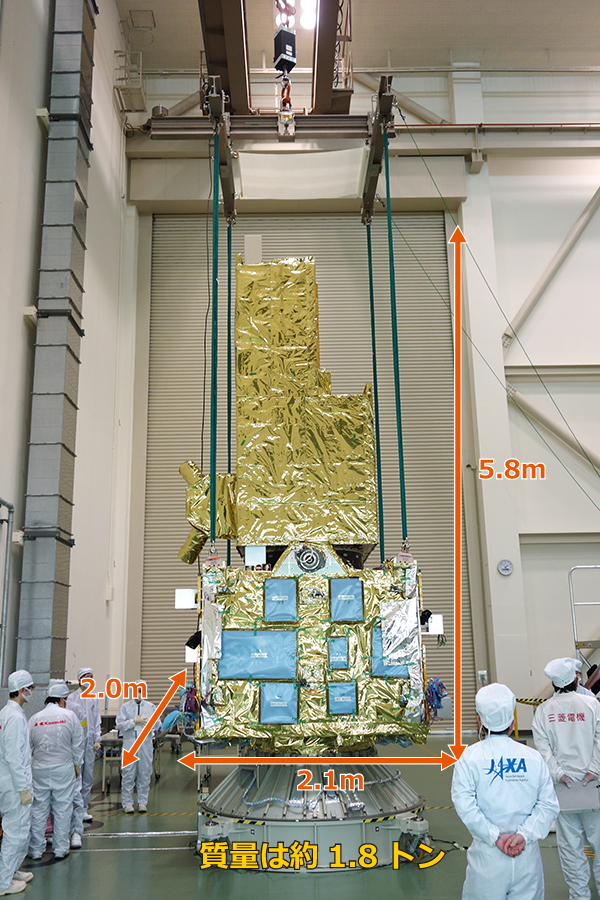
\includegraphics[width=0.9\columnwidth]{./figure/大型.jpg}
        \caption{大型人工衛星}
        \label{fig:c}
    \end{minipage}
\end{figure}
    


 人工衛星は,地球との通信のためのアンテナや,発電のための太陽光パネルの向きを制御するために,姿勢の制御が行われる.
なお,ここでいう「姿勢」とは,人工衛星内に選んだ基準軸と特定の基準座標系との関係をいう\cite{intro3}.
人工衛星の姿勢制御の方式には,主に以下のようなものがある.

\begin{itemize}
    \item 重力傾度姿勢安定方式\\
    軌道を廻る衛星が地球の重力により衛星の軸のうち一つが常に地球の中心を向く性質を利用するもの.
    能動的な制御やエネルギーを必要としない\cite{intro4}.
    \item スピン安定方式\\
    慣性主軸の回りにスピンを与えて,コマのように安定させる方式.衛星全体を回転させるシングルスピン方式と,
    通信用のアンテナを回転させないため,アンテナ部と衛星本体をそれぞれ違う方向に回転させるデュアルスピン方式がある\cite{intro5}.
    \item 3軸安定方式\\
    衛星の直交する3軸(ロール・ピッチ・ヨー角)の各軸について制御する方式である.
    リアクションホイールを用いるものには,ジャイロ効果を用いるバイアスモーメンタム方式と,
    外乱に応じて回転数を変化させるゼロモーメンタム方式がある\cite{intro5}.
\end{itemize}

 特に3軸安定方式に用いられるアクチュエータには,スラスター,リアクションホイール,
コントロールモーメントジャイロ(Control Moment Gyroscopes: CMG),磁気トルカといったものがある.
スラスターは,推進剤を噴出し,その反力で推進力を得るものである.
またリアクションホイールは,ホイールを回転させて生ずる反力によるトルクで回転を起こし,
CMGは,その回転の向きを変えることにより姿勢を制御する.
磁気トルカは,電磁誘導を利用してコイルに発生させた磁気モーメントと
地磁気を反応させることでトルクを発生させ,回転力を得るものである.
超小型人工衛星は,その小ささから,搭載可能な機器のサイズや重量に制限がある.
そのため,リアクションホイールやスラスタといった,性能の代わりに大型な機器は搭載が難しい.
そこで,姿勢制御に磁気トルカやCMG(コントロールモーメントジャイロ)が用いられることが多い.
図\ref{fig:act}に,人工衛星の姿勢制御によく用いられるアクチュエータの例を示す.

\begin{figure}[H]
	\centering
		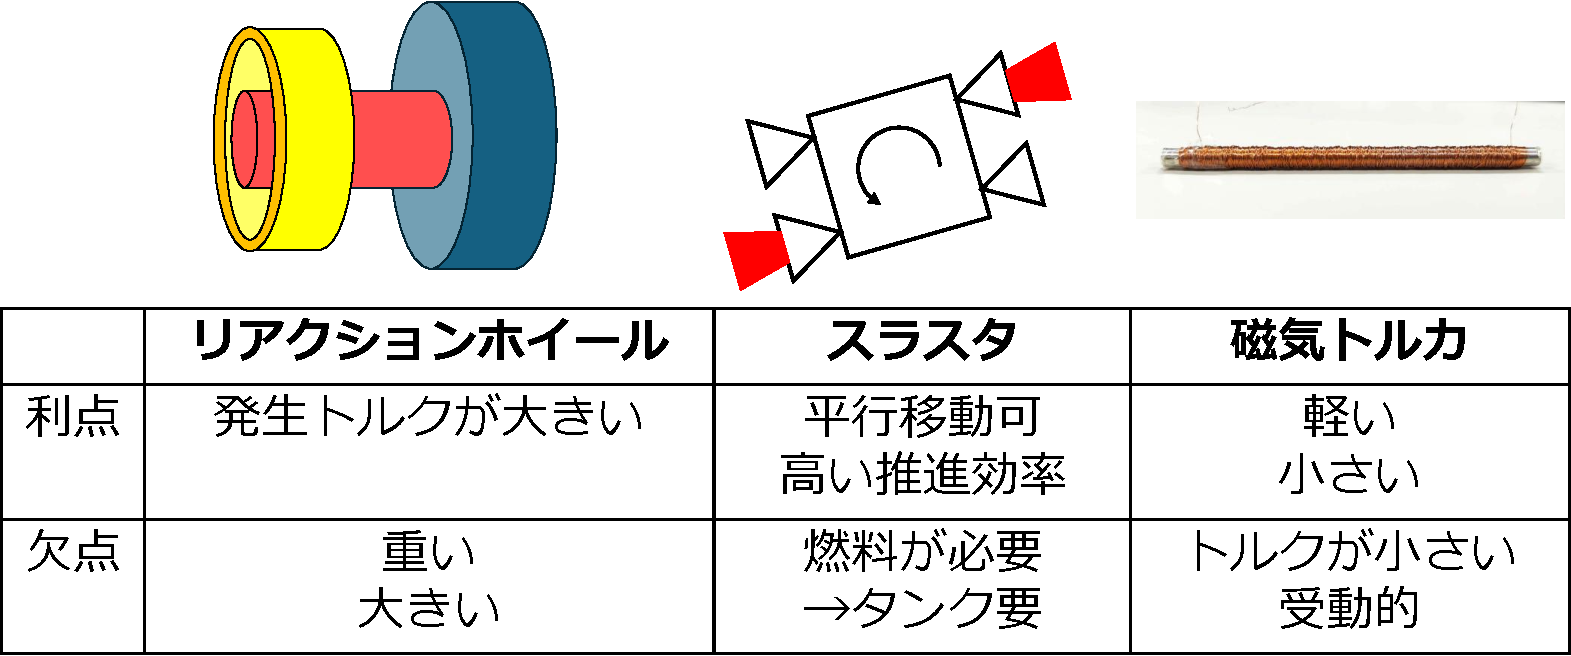
\includegraphics[scale=0.5]{./figure/序論図-crop.pdf}
		\caption{アクチュエータの例}
		\label{fig:act}
\end{figure}

\subsection{本研究の目的}
 人工衛星の姿勢制御を地上で実験し,研究・検討するには,通常球面の空気軸受けを使った3軸テーブルが用いられる.
しかし,3軸で制御する衛星でも,3軸を同時に検証する前に,1軸のみでの制御実験を検証する場合が多い\cite{intro6}.
また,3軸での実験の設計の難しさから,1軸での実験装置は有効な実験道具となる.

 本研究では,小型衛星の模型を用いて,磁気トルカを用いて1軸のみの衛星の姿勢制御を行う様子を再現し,
人工衛星によく用いられる,B-dot制御則やクロスプロダクト則といった制御理論や,P制御,PD制御といった基本的な理論を検証する.
実際の人工衛星の動きを完璧にトレースするのではなく,あくまでもデモンストレーションとして,制御理論の特徴を反映できることを確かめる.

 本論文の構成は,2章で検証する制御理論についてまとめ,3章で作製した実験システムについてまとめ,4章で検証の手法,結果を示し,考察を行い,最後に5章で本研究のまとめを示している.